\chapter{Pipelines}
\section{Embedding-Decoupled Strategies, e.g., Graph2Vec}

The Graph2Vec-based pipeline follows an \emph{embedding-decoupled} design, in which the representation learning stage and the forecasting stage are trained independently and communicate only through a fixed-dimensional embedding vector. This decoupling is the defining property of the family of strategies analysed in this section: the graph encoder has no access to the downstream forecasting loss, and the forecaster treats the embeddings as static exogenous features. Figure~\ref{fig:graph2vec-comparison} summarises the resulting two-stage architecture, which can be decomposed into an offline \emph{Graph2Vec pipeline} and an online \emph{LSTM forecasting pipeline}.

\paragraph{Offline stage --- Graph2Vec pipeline.}
The first stage operates on a multivariate panel of all item-level time series. For every item \(i\), the historical demand is z-score normalized using a \texttt{StandardScaler} fitted exclusively on the training window of that item, ensuring that no information from the validation or test periods leaks into the graph construction. A sliding window of width \(w=15\) and stride \(s=1\) was then applied to the scaled series, producing, at each timestamp \(t\), a snapshot of the cross-sectional dynamics over the interval \([t-w+1,t]\).

For each window, a \emph{similarity graph} \(G_t=(V,E_t)\) is built, where the node set \(V\) corresponds to the items in the catalogue, and the edge set \(E_t\) encodes pairwise relationships between their windowed sub-series. Edges are instantiated whenever a chosen similarity or distance metric, such as Spearman, Pearson, Kendall, DTW, CID, SBD, or Catch22, exceeds a fixed threshold, which is considered a grid-search hyperparameter. The resulting sequence \(\{G_t\}_{t=1}^{T}\) captures how the inter-item relational structure evolves over time while keeping the node identity stable across windows.

Each graph \(G_t\) is subsequently passed to a \textbf{Graph2Vec} model~\cite{narayanan2017graph2vec}, which combines the Weisfeiler--Lehman (WL) relabelling scheme with a Doc2Vec skip-gram objective. The WL procedure produces, for each graph, a multiset of rooted subtree patterns that serves as the analog of a ``document''; Doc2Vec then learns a continuous representation \(z_t \in \mathbb{R}^{d}\), with \(d=20\) in our configuration, such that graphs sharing similar substructures are mapped to nearby points in the embedding space. Crucially, this stage is fully \emph{unsupervised} with respect to the forecasting task: it has no access to the target variable beyond the unsupervised similarity structure used to construct the edges.

Therefore, the output of the offline stage is a temporally indexed sequence of graph embeddings \(\{z_t\}\), which is computed once and cached on the disk. Whenever the same metric, threshold, and window configuration are required again, the embeddings are loaded from the disk rather than recomputed, which makes the systematic grid search tractable.

\paragraph{Online stage --- LSTM forecasting pipeline.}
The second stage consumes the cached embeddings as additional input channels to an LSTM forecaster trained per item--store pair. Three families of features were concatenated at each time step as follows:

\begin{enumerate}
    \item the \emph{target series} for the focal item, MinMax-scaled on the training window;
    \item a set of \(28\) \emph{exogenous calendar features}, including day-of-week, month, week-of-year, holiday, and pre-/post-holiday indicators, also MinMax-scaled;
    \item the corresponding \emph{graph embedding} \(z_t \in \mathbb{R}^{20}\), aligned in time with the focal series so that the embedding observed at step \(t\) reflects only information available up to \(t\).
\end{enumerate}

This yields, for a sequence length of \(L=30\), an input tensor of shape \((L,1+28+20)=(30,49)\). The tensor is fed to an LSTM with a single recurrent layer, hidden size \(32\), and \texttt{batch\_first=True}; the last hidden state is passed through a dropout layer and a linear projection \(\mathbb{R}^{32} \to \mathbb{R}^{1}\) to produce the one-step-ahead forecast, which is finally inverse-scaled to the original demand units. Optimization uses Adam with a learning rate of \(10^{-3}\), up to \(1000\) epochs, and early stopping with a patience \(100\) on the validation loss.

\begin{figure}[htbp]
    \centering

    \begin{subfigure}[t]{0.48\linewidth}
        \centering
        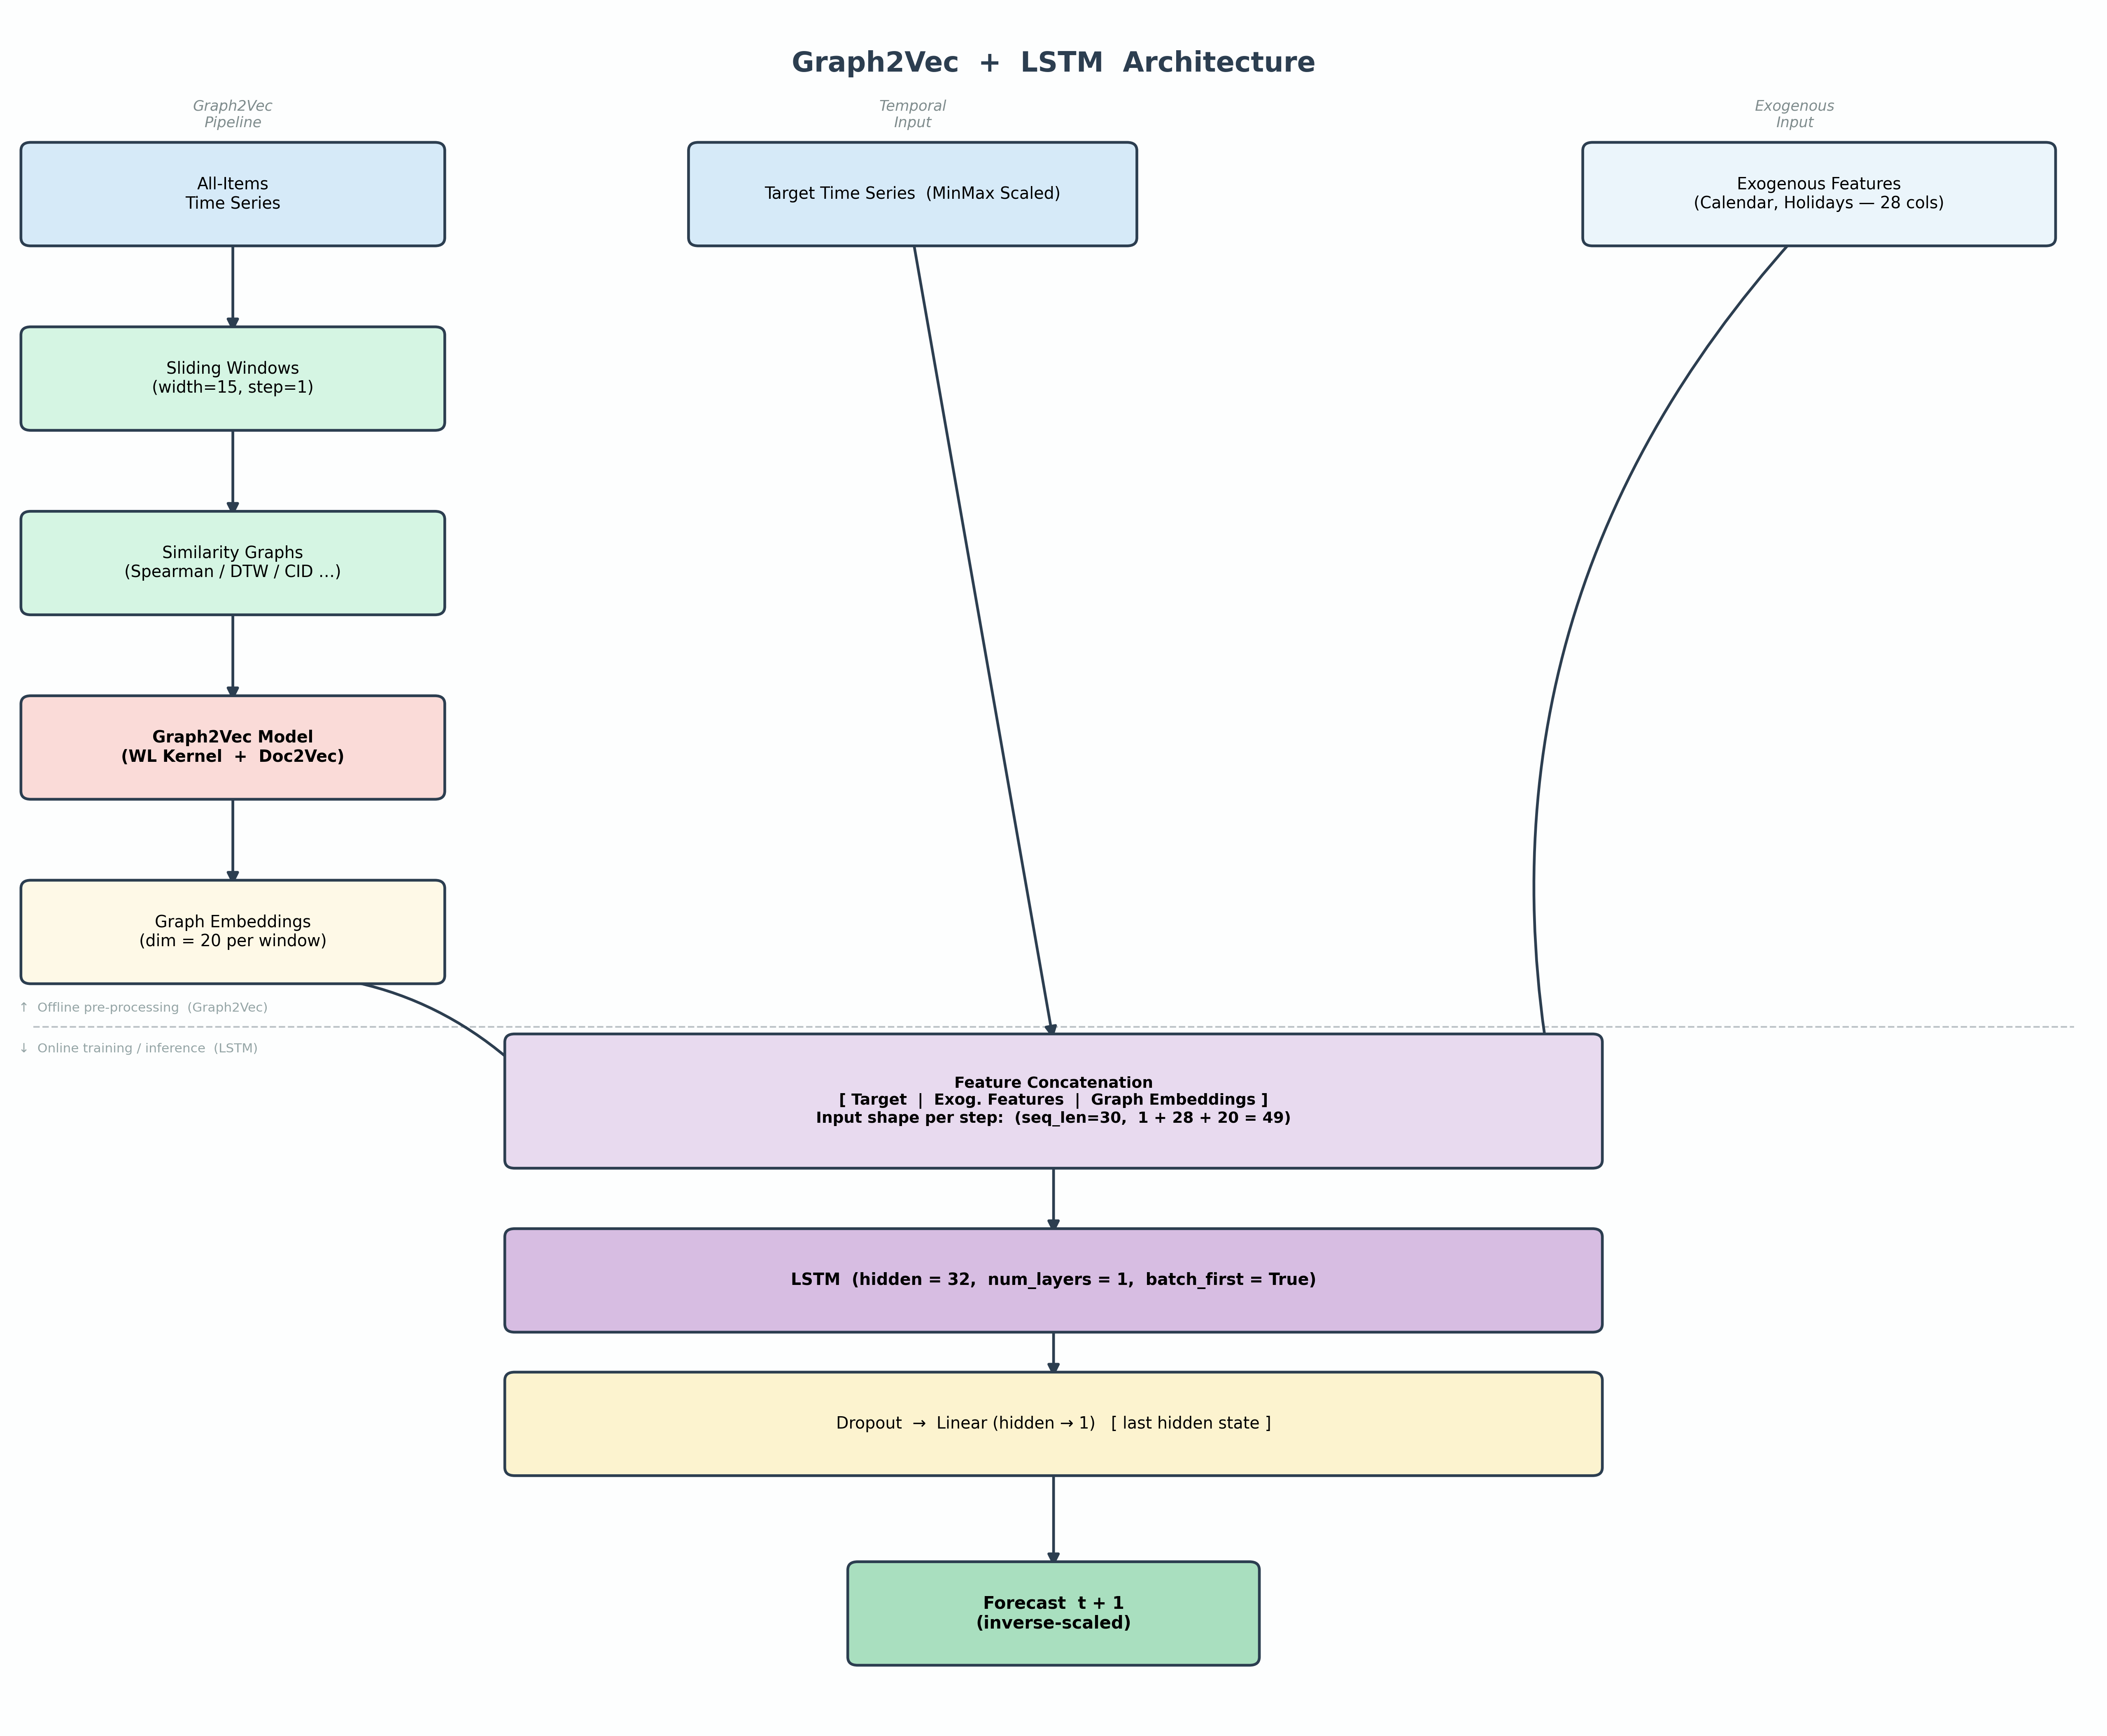
\includegraphics[width=\linewidth]{figures/Graph2VecLSTM.png}
        \caption{Graph2Vec-LSTM architecture.}
        \label{fig:graph2vec-lstm}
    \end{subfigure}
    \hfill
    \begin{subfigure}[t]{0.48\linewidth}
        \centering
        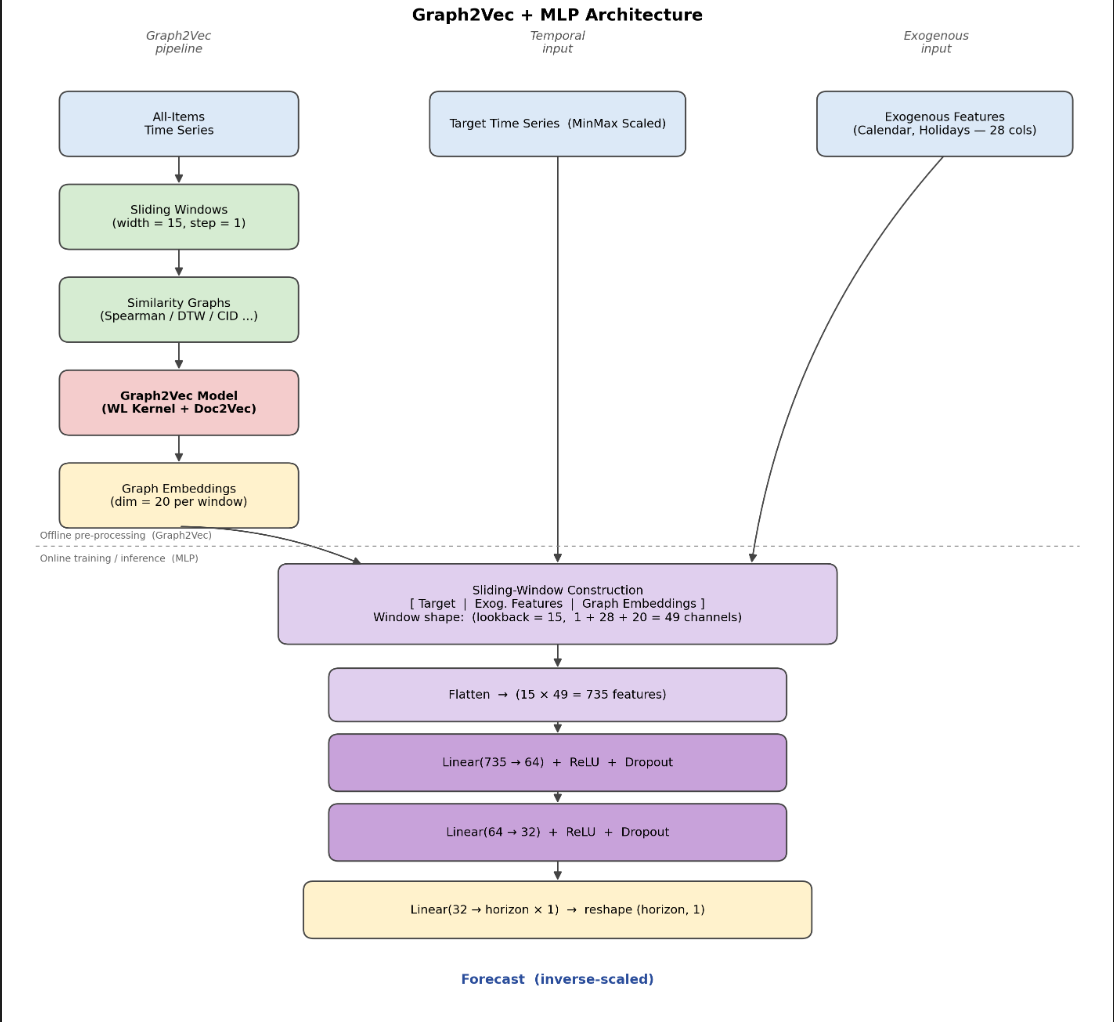
\includegraphics[width=\linewidth]{figures/Graph2Vec_MLP.png}
        \caption{Graph2Vec-MLP architecture.}
        \label{fig:graph2vec-mlp}
    \end{subfigure}

    \caption{Comparison of the Graph2Vec-based forecasting architectures.}
    \label{fig:graph2vec-comparison}
\end{figure}


To isolate the contribution of the relational signal, a \emph{no-embedding} baseline is run alongside every embedding configuration, using exactly the same target and exogenous features but with the embedding channel removed, providing an input size of \(1+28=29\). For each item--store--seed triplet, the grid search jointly varied the similarity metric and edge threshold while keeping the window size, step size, and LSTM hyperparameters fixed. Multiple seeds, such as \(42\), \(1000\), \(26008\), and \(213626\), were evaluated to characterize the variability of the results.


\section{GNN-Based End-to-End Strategies}

GNN-based end-to-end strategies have been designed to incorporate relational information directly into the forecasting process. Instead of relying only on the historical demand of an individual product, these approaches represent each target product as part of a dynamic graph, where the neighboring nodes correspond to products with similar temporal behaviors. This allows the model to learn not only from the target product's own demand pattern but also from the demand evolution of related products.

The main motivation for this strategy is that product demand is often influenced by shared patterns across items, such as common seasonality, similar sales cycles, category-level behavior, or correlated responses to calendar effects. A purely sequential model, such as an LSTM, or a purely feature-based model, such as an MLP, may fail to explicitly capture these relationships. Using a graph neural network, the forecasting model can aggregate information from similar products and learn a representation that reflects both temporal and structural dependencies.

In this study, a GNN-based strategy was implemented as an end-to-end hybrid architecture. The graph component learns a representation of the target product from its ego-graph, whereas the forecasting component combines this graph representation with the target product's recent time-series window and exogenous calendar features. The complete model is trained directly with the forecasting objective, meaning that the graph representation is optimized to improve the prediction accuracy rather than being computed as a separate, fixed embedding.

During inference, the model follows a recursive-forecasting procedure. At each step, the most recent demand window is used to rebuild the graph, the model predicts the next value, and the prediction is appended to the input window for the next step. This process allows the graph structure and temporal input to evolve throughout the multi-step forecast horizon, making the approach suitable for dynamic demand-forecasting scenarios.

\subsection{GCN}

A Graph Convolutional Network (GCN) is used as the graph-learning component of the proposed end-to-end hybrid strategy. For each target product, an ego graph is constructed by connecting the target node to other products whose historical demand patterns are considered similar according to a selected similarity or distance metric. The target product is always represented as the central node, whereas the neighboring nodes provide additional contextual information about the related demand behavior.

Each node in the graph contains time-series features extracted from a sliding window. Edges between nodes are weighted according to the similarity score between products. Therefore, stronger relationships have a greater influence during the graph convolution process.

The GCN branch applies graph convolutional layers to propagate and aggregate information across the ego-graph. Through this process, the representation of the target node is updated using information from its neighbouring products. The resulting target-node embedding captures relational demand patterns that are not available when modelling the target series in isolation.

This graph-based embedding is then combined with a separate temporal representation of the target product. The temporal branch receives the recent lookback window together with exogenous variables, such as calendar-related features, and projects them into a latent representation. The GCN embedding and the temporal projection are normalised, concatenated, and passed through an MLP prediction head to produce the next-step forecast.

The role of the GCN is therefore to enrich the forecasting model with information from structurally related products. By learning from both the target product and its dynamically selected neighbours, the model can better capture shared demand patterns and improve robustness in cases where the individual time series is noisy, sparse, or affected by irregular fluctuations.

\subsection{Node Feature Computation}

A central design choice in the GCN branch concerns how each node in the
ego-graph is described, since the node features determine what information
the graph convolution propagates and aggregates. In every configuration, the
features are extracted from the same sliding window of raw demand used to
construct the graph: given a window of width $W$, each node $i$ is associated
with its demand sub-sequence $\mathbf{x}_i \in \mathbb{R}^{W}$ over that
window. The way this sub-sequence is transformed into a node-feature vector
defines three alternative representations that were investigated in this work:
the raw demand sequence, an eight-dimensional statistical summary, and the
\textit{catch22} feature set. All three operate on a node-by-node basis and
produce a feature matrix of shape $(n_\text{nodes} \times d)$, where $d$ depends
on the chosen representation.

\subsubsection{Raw Demand Sequence}

The simplest representation uses the demand window itself as the node feature,
so that $d = W$ and the feature vector of node $i$ is exactly its raw
sub-sequence $\mathbf{x}_i$. This preserves the full temporal resolution of
each node and lets the GCN operate directly on the local demand trajectory of
the target product and its neighbours, without any hand-crafted aggregation.
The trade-off is that the feature dimensionality grows with the window length
and the representation contains no explicit notion of trend, dispersion, or
shape; any such structure must be recovered implicitly by the graph
convolution. It also makes the node features sensitive to the absolute scale
and length of the window, which can be advantageous when magnitude carries
information but detrimental when the relevant signal is the shape of the
series rather than its level.

\subsubsection{Eight-Dimensional Statistical Summary}

The second representation replaces the raw window with a compact set of eight
descriptive statistics computed over each node's sub-sequence:
\[
\mathbf{f}_i = \big[\,\mu_i,\; \sigma_i,\; \min_i,\; \max_i,\; x_i^{(0)},\;
x_i^{(W-1)},\; s_i,\; \Sigma_i \,\big],
\]
where $\mu_i$ and $\sigma_i$ are the mean and standard deviation of the window,
$\min_i$ and $\max_i$ its extrema, $x_i^{(0)}$ and $x_i^{(W-1)}$ the first and
last observed values, $\Sigma_i$ the sum over the window, and
\[
s_i = \frac{x_i^{(W-1)} - x_i^{(0)}}{\max(W-1,\,1)}
\]
a simple slope capturing the net direction of change across the window. This
representation produces a fixed eight-dimensional feature vector regardless of
the window length, summarising the level (mean, sum, extrema), dispersion
(standard deviation, range) and short-term trend (first/last values, slope) of
each product's recent demand. It is markedly more compact than the raw
sequence and encodes interpretable demand characteristics directly, at the cost
of discarding the fine-grained temporal ordering within the window.

\subsubsection{catch22 Features}

The third representation draws on \textit{catch22} (CAnonical Time-series
CHaracteristics) \cite{lubba2019catch22canonicaltimeseriescharacteristics}, a curated set of 22 features selected for their
discriminative power and low mutual redundancy across diverse time-series
classification tasks. These features summarise higher-order temporal properties
of each window, such as autocorrelation structure, distribution shape,
entropy, linear and nonlinear predictability, and measures of stationarity,
yielding a $22$-dimensional descriptor per node. Because \textit{catch22}
internally z-normalises each series before extracting its shape and dynamics
features, all information about the absolute scale of the demand is, by design,
discarded. To recover this scale information, an extended $24$-dimensional
variant (\textit{catch24}) was also used, which appends the mean
(\texttt{DN\_Mean}) and the standard deviation (\texttt{DN\_Spread\_Std}) of
the raw window to the 22 shape features.

This representation nonetheless requires a numerical safeguard, because several
\textit{catch22} features become mathematically ill-defined on short or
near-constant windows and return \texttt{NaN}, while strictly constant series
can additionally fail in the underlying feature-extraction backend. Although the
selected products were chosen among the best-selling smooth and erratic items,
both of which exhibit frequent demand occurrences and are therefore unlikely to
produce long runs of zeros within a window, such degenerate windows can still
arise occasionally and must be handled robustly. To prevent a single degenerate
node from corrupting the entire graph during message passing, any feature that
is undefined or non-finite is replaced by zero, and a node whose extraction
fails entirely falls back to an all-zero feature vector. Relative to the
eight-dimensional summary, the \textit{catch22} representation captures
substantially richer temporal dynamics while keeping a fixed,
window-length-independent dimensionality, at the cost of higher extraction
complexity and reduced interpretability of the individual features.

Regardless of the chosen representation, the node features are recomputed
dynamically as the graph evolves. During the recursive multi-step forecast,
the target node's feature row is refreshed at each step from the rolling demand
window, where the most recent observation is replaced by the model's own
prediction rather than the ground-truth value. The same feature transformation
used during training is therefore applied consistently at inference time,
ensuring that no test-period information leaks into the node features while the
graph structure and node descriptors are updated throughout the forecast
horizon.
\subsubsection{Link to LSTM Training}

The GCN and the LSTM are not trained as separate stages. Instead, they form a
single end-to-end network in which the graph encoder, the recurrent encoder,
and the prediction head are optimised jointly under one forecasting loss. The
GCN does not produce a fixed, precomputed embedding; rather, its parameters are
updated by the same gradient signal that trains the LSTM, so that the learned
graph representation is shaped specifically to improve the forecast.

\paragraph{Per-step coupling of the two branches.}
The two branches are coupled at every step of the lookback window. For a
lookback length $L$, each training sample carries $L$ ego-graphs, one per
lookback day, aligned so that the graph used at step $i$ is built strictly from
the days preceding it (preventing label leakage). During a forward pass, a
batch of $B$ samples is flattened into $B \times L$ ego-graphs and encoded by
the GCN in a single sparse operation. Two graph-convolutional layers propagate
information across each ego-graph, and the embedding of the target node (row $0$
of every subgraph, recovered through the batch pointer indices) is extracted
and passed through a layer normalisation, yielding a per-step graph vector
$\mathbf{z} \in \mathbb{R}^{d_g}$. These vectors are reshaped back to
$(B, L, d_g)$ in the same row-major order produced by the collation step, so
that each lookback day is paired with the graph embedding computed for that day.

\paragraph{Fusion before the recurrence.}
The graph embedding is fused with the temporal input \emph{before} the LSTM
processes the sequence. At each step the model concatenates the target value,
the exogenous calendar features, and the corresponding graph embedding into a
single augmented vector,
\[
\mathbf{x}_t = \big[\, y_t \;\Vert\; \mathbf{e}_t \;\Vert\; \mathbf{z}_t \,\big]
\in \mathbb{R}^{1 + n_\text{exog} + d_g},
\]
and the resulting sequence $(\mathbf{x}_1, \dots, \mathbf{x}_L)$ is fed to the
LSTM. Because the relational signal enters the recurrence as additional
input features at every step, the LSTM can integrate structural information
from related products together with the target's own temporal dynamics, rather
than treating the graph embedding as a static side input. The hidden state of
the final step is passed through dropout and a linear head to produce the
next-step prediction.

\paragraph{Backpropagation through both branches.}
Training minimises a single forecasting loss (mean squared error) between the
final-step prediction and the ground-truth target, with mean absolute error
used for validation and early stopping. The optimiser is bound to all model
parameters at once, so a single call to backpropagation propagates gradients
from the prediction head, back through the LSTM, through the concatenation that
fused the two branches, and into the GCN convolutional layers and the layer
normalisation. The concatenation is the point at which the error signal splits:
part of it flows along the temporal path into the LSTM weights, and part flows
along the structural path into the GCN weights and, through the edge-weighted
message passing, shapes how neighbour information is aggregated. The graph
representation is therefore learned discriminatively for the forecasting
objective, not as an unsupervised or pretext embedding.

\paragraph{Training stabilisation and diagnostics.}
Several mechanisms keep the joint optimisation stable. Layer normalisation on
$\mathbf{z}$ prevents the magnitude of the graph embedding from dominating or
collapsing relative to the temporal features at the fusion point. Global
gradient-norm clipping bounds the combined gradient before each optimiser
update, and dropout is applied in the GCN, the LSTM, and the head to limit
overfitting. To monitor the relative contribution of the two branches during
training, the loop separately accumulates the gradient norms of the
graph-related parameters (the convolutional layers and $\mathbf{z}$
normalisation) and of the LSTM parameters, and logs their ratio together with
the mean norm and variance of the captured $\mathbf{z}$ embeddings. These
diagnostics make it possible to verify that the graph branch is actually
receiving and using a meaningful share of the learning signal rather than being
ignored. An ablation switch is also provided that zeroes the graph embedding
before fusion, reducing the architecture to a purely temporal LSTM and allowing
the contribution of the GCN branch to be measured directly.

\paragraph{Recursive inference.}
Since the model forecasts a single step ahead, multi-step predictions are
generated by recursive roll-out. At inference the model maintains a rolling
deque of $L$ ego-graphs alongside the $L$-row lookback window, mirroring the
per-step layout used during training. At each step it is queried on the current
(\,$L$-graph deque, $L$-row temporal window\,) pair to predict the next value
$\hat{y}$; the lookback window is then advanced by dropping the oldest target
value and appending $\hat{y}$, while the exogenous row is moved to the calendar
features of the day being predicted, and the graph deque is advanced by dropping
the oldest graph and appending the ego-graph aligned to that same day. Both the
temporal input and the underlying graph structure therefore evolve jointly
across the horizon rather than being held fixed. To keep the forecast strictly
causal and free of label leakage, the target node's feature row of each newly
appended graph is recomputed from a rolling window of the model's \emph{own}
predictions, where $\hat{y}$ is inverse-scaled, re-scaled with the target
product's scaler, and used to regenerate the node features through the same
transformation chosen at training time (the raw sequence, the eight-dimensional
summary, or the \textit{catch22} descriptor); the same own-prediction history
is used to refresh any leakage-prone exogenous features such as demand lags and
rolling means. The predictions are finally inverse-transformed back to the
original demand scale, so the GCN+LSTM is rolled out autoregressively while
preserving identical, causal train- and test-time semantics over the entire
forecast horizon.
\subsubsection{Link to MLP Training}
\label{sec:gcn_mlp_link}

As in the recurrent variant, the GCN and the MLP are not trained as separate
stages. They form a single end-to-end network, \texttt{SimpleGCNMLPForecaster},
in which the graph encoder, a shared time-distributed MLP, and the prediction
head are optimised jointly under one forecasting loss. The GCN does not produce
a fixed, precomputed embedding; its parameters are updated by the same gradient
that trains the MLP, so the learned graph representation is shaped specifically
to improve the forecast.

\paragraph{Per-step coupling of the two branches.}
The two branches are coupled at every step of the lookback window. For a
lookback length $L$, each training sample carries $L$ ego-graphs, one per
lookback day, aligned so that the graph used at step $i$ is built strictly from
the days preceding it (preventing label leakage). During a forward pass, a
batch of $B$ samples is flattened into $B \times L$ ego-graphs and encoded by
the GCN in a single sparse operation. Two edge-weighted graph-convolutional
layers (with self-loops, ReLU and dropout in between) propagate information
across each ego-graph, and the embedding of the target node (row $0$ of every
subgraph, recovered through the batch pointer indices) is extracted and passed
through a layer normalisation, yielding a per-step graph vector
$\mathbf{z}_t \in \mathbb{R}^{d_g}$. These vectors are reshaped back to
$(B, L, d_g)$ in the same row-major order produced by the collation step, so
that each lookback day is paired with the graph embedding computed for that day.

\paragraph{Fusion before the head.}
The graph embedding is fused with the temporal input \emph{per step}, before
the MLP processes the sequence. At each step the model concatenates the target
value, the exogenous calendar features, and the corresponding graph embedding
into a single augmented vector,
\[
\mathbf{x}_t = \big[\, y_t \;\Vert\; \mathbf{e}_t \;\Vert\; \mathbf{z}_t \,\big]
\in \mathbb{R}^{1 + n_\text{exog} + d_g},
\]
giving an augmented sequence $(\mathbf{x}_1, \dots, \mathbf{x}_L)$. Crucially,
this sequence is \emph{not flattened} into one long vector, and there is no
separate linear projection of the lookback: the relational signal enters as
additional per-step features, exactly as in the recurrent variant, the only
difference being how the augmented sequence is subsequently consumed.

\paragraph{Time-distributed MLP head.}
Instead of a recurrence, a single shared MLP (a stack of
\texttt{Linear $\to$ ReLU $\to$ Dropout} blocks) is applied independently and
with identical weights to each of the $L$ augmented steps, mapping
$\mathbf{x}_t \mapsto \mathbf{h}_t$. This time-distributed design keeps the
head invariant to the lookback length and lets the network learn one per-step
transformation that is reused across the window, rather than learning a
position-specific mapping over a flattened input. The $L$ step
representations are then pooled by concatenating the most recent step with the
mean over all steps,
\[
\mathbf{g} = \big[\, \mathbf{h}_L \;\Vert\; \tfrac{1}{L}\textstyle\sum_{t=1}^{L}\mathbf{h}_t \,\big],
\]
combining the latest local context with a global summary of the window, and a
final linear layer maps $\mathbf{g}$ to the forecast horizon $H$.

\paragraph{Backpropagation through both branches.}
Training minimises a single forecasting loss (e.g.\ mean squared error) between
the final-step prediction and the ground-truth target, with a separate metric
used for validation and early stopping. The optimiser is bound to all model
parameters at once, so a single backward pass propagates gradients from the
linear head, back through the pooled representation and the shared per-step MLP,
through the concatenation that fused the two branches, and into the GCN
convolutional layers and the layer normalisation. The concatenation is the
point at which the error signal splits: part flows along the temporal path into
the MLP weights, and part flows along the structural path into the GCN weights
and, through the edge-weighted message passing, shapes how neighbour
information is aggregated. The graph representation is therefore learned
discriminatively for the forecasting objective, not as an unsupervised or
pretext embedding.

\paragraph{Training stabilisation and diagnostics.}
The same stabilisation mechanisms as the recurrent variant apply. Layer
normalisation on $\mathbf{z}$ prevents the magnitude of the graph embedding
from dominating or collapsing relative to the temporal features at the fusion
point. Global gradient-norm clipping bounds the combined gradient before each
optimiser update, and dropout is applied in both the GCN and the MLP. To
monitor the relative contribution of the two branches, the training loop
separately accumulates the gradient norms of the graph-related parameters
(the convolutional layers and the $\mathbf{z}$ normalisation) and of the MLP
parameters, and logs their ratio together with the mean norm and variance of
the captured $\mathbf{z}$ embeddings, verifying that the graph branch receives
a meaningful share of the learning signal. An ablation switch is also provided
that zeroes the graph embedding before fusion, reducing the architecture to a
purely temporal time-distributed MLP and allowing the GCN contribution to be
measured directly.

\paragraph{Recursive inference.}
At test time the fused model is rolled out one step at a time. A deque of $L$
ego-graphs is maintained alongside the lookback window: at each step the model
predicts the next value, the prediction is appended to the lookback (and to the
unscaled history used for any leakage-safe lag and rolling-mean features), and
the graph deque is advanced by dropping the oldest graph and appending the
graph aligned to the day just predicted. To avoid label leakage, the target
node's feature row in each newly appended graph is overwritten with features
derived from the model's own rolling predictions rather than ground-truth test
values. The same forward signature
$\texttt{model}(G_t, \mathbf{s}_t) \rightarrow (B, H, 1)$ is used during
training and inference, so train- and test-time semantics are identical and the
graph information is exploited consistently throughout the forecast horizon.



